\documentclass[11pt]{article}
\usepackage{multicol}
\usepackage{ifthen}
%\usepackage{multitoc}
%\usepackage{german}
%\usepackage{bibgerm}
\usepackage{amsmath}
\usepackage{amsfonts}
\usepackage{color}
\usepackage{hyperref}
\usepackage[dvips]{epsfig}
\usepackage{subfigure}
\usepackage[dvips]{graphicx}
\usepackage[a4paper,body={148mm,240mm,nohead}]{geometry}
\usepackage[ansinew]{inputenc}
\usepackage{listings}
\lstset{language=C++, basicstyle=\ttfamily,
  stringstyle=\ttfamily, commentstyle=\it, extendedchars=true}

\newif\ifpdf
\ifnum\ifx\pdfoutput\undefined0\else\pdfoutput\fi<1
\pdffalse % we are not running PDFLaTeX
\else
\pdftrue % we are running PDFLaTeX
\fi

\ifpdf
\usepackage[pdftex]{graphicx}
\else
\usepackage{graphicx}
\fi

\ifpdf
\DeclareGraphicsExtensions{.pdf, .jpg, .tif}
\else
\DeclareGraphicsExtensions{.eps, .jpg}
\fi

\newcommand{\C}{\mathbb{C}}
\newcommand{\R}{\mathbb{R}}
\newcommand{\N}{\mathbb{N}}
\newcommand{\Z}{\mathbb{Z}}
\newcommand{\Q}{\mathbb{Q}}
\newcommand{\K}{\mathbb{K}}


\title{Iterative Solver Template Library\thanks{Part of the
    Distributed and Unified Numerics Environment (DUNE) which is
    available from the site
    \url{http://www.dune-project.org/}}}

\author{%
Peter Bastian, Markus Blatt\\
Institut f\"ur parallele und verteilte Systeme (IPVS),\\
Universit\"at Stuttgart, Universit\"atsstr. 38, D-70569 Stuttgart, \\
email: \texttt{Peter.Bastian@ipvs.uni-stuttgart.de}, \texttt{Markus.Blatt@ipvs.uni-stuttgart.de}}

\date{April 13, 2007}

\begin{document}

\maketitle

\begin{abstract}
This document describes the rationale behind and use of the Iterative
Solver Template Library (ISTL) which provides a set of C++
templates to represent vectors, (sparse) matrices and some generic
algorithms based on these. The most prominent features of the
matrix/vector classes is that they support a recursive block structure
in a bottom up way. The classes can be used, e.~g., to efficiently implement
block preconditioners for $hp$-finite elements.
\end{abstract}

\begin{multicols}{2}
{\small\tableofcontents}
\end{multicols}

\section{Introduction}

The numerical solution of partial differential equations (PDEs) frequently requires the
solution of large and sparse linear systems. Naturally,
there are many libraries available on the internet for doing sparse matrix/vector
computations. A comprehensive overview is given in \cite{LALinks}. 

The
widely availably Basic Linear Algebra Subprograms (BLAS) standard has
been extended to cover als sparse matrices \cite{BLASTForum}. BLAS
divides the available functions into level 1 (vector operations),
level 2 (vector/matrix operations) and level 3 (matrix/matrix
operations). BLAS for sparse matrices contains only level 1 and 2
functionality and is quite different to the standard for dense
matrices. The standard uses procedural programming style and offers
only a FORTRAN and C interface. As a consequence, the interface is
``coarse grained'', meaning that ``small'' functions such as access to
individual matrix elements is relatively slow. 

Generic programming techniqes in C++ offer the possibility to combine
flexibility and reuse (``efficiency of the programmer'') with fast
execution (``efficieny of the program'') as has been demonstrated with
the Standard Template Library (STL), \cite{Stroustrup} or the Blitz++
library for multidimensional arrays \cite{Blitz}. A variety of
template programming techniques such as traits, template metaprograms,
expression templates or the Barton-Nackman trick are used in the
implementations, see \cite{BN,Veldhui99} for an introduction.
Application of these ideas to matrix/vector operations is available
with the Matrix Template Library (MTL), \cite{MTL,MTL_SciTools98}. The Iterative
Template Library (ITL), \cite{ITL}, implements iterative solvers for
linear systems (mostly Krylov subspace methods) in a generic way based
on MTL. The Distributed and Unified Numerics Environment (DUNE),
\cite{Dune,DuneWeb}, applies the STL ideas to finite element
computations. 

Why bother with yet another OO-implementation of (sparse) linear
algebra when libraries, most notably the MTL, are available? The most
important reason is that the functionality in existing libraries has
not been designed specifically with advanced finite element methods in
mind. Sparse matrices in finite element computations have a lot of
structure. Here are some examples:
\begin{itemize}
\item Certain discretizations for systems of PDEs or higher order
  methods result in matrices where individual entries are replaced by
  small blocks, say of size $2\times 2$ or $4\times 4$, see
  Fig. \ref{fig:festructure}(a).  Dense blocks of different sizes
  e.~g. arise in $hp$ Discontinuous Galerkin discretization methods,
  see Fig. \ref{fig:festructure}(b). Straightforward
  iterative methods solve these small blocks exactly, see
  e.~g.~\cite{BH99}.
\item Equation-wise ordering for systems results in matrices having an
  $n\times n$ block structure where $n$ corresponds to the number of
  variables in the PDE and the blocks themselves are large, see Fig.
  \ref{fig:festructure}(d). As an
  example we mention the Stokes system. Iterative solvers such as the
  SIMPLE or Uzawa algorithm use this structure.
\item Other discretizations, e.~g. those of reaction/diffusion
  systems,  produce sparse matrices whose blocks are
  sparse matrices of small dense blocks, see fig. \ref{fig:festructure}(c).
\item Other structures that can be exploited are the level structure
  arising from hierarchic meshes, a p-hierarchic
  structure (e.~g.~decomposition in linear and quadratic part),
  geometric structure from decomposition in subdomains or topological
  structure where unknowns are associated with nodes, edges, faces or
  elements of a mesh.
\end{itemize}
\begin{figure}[htb]
  \centering
  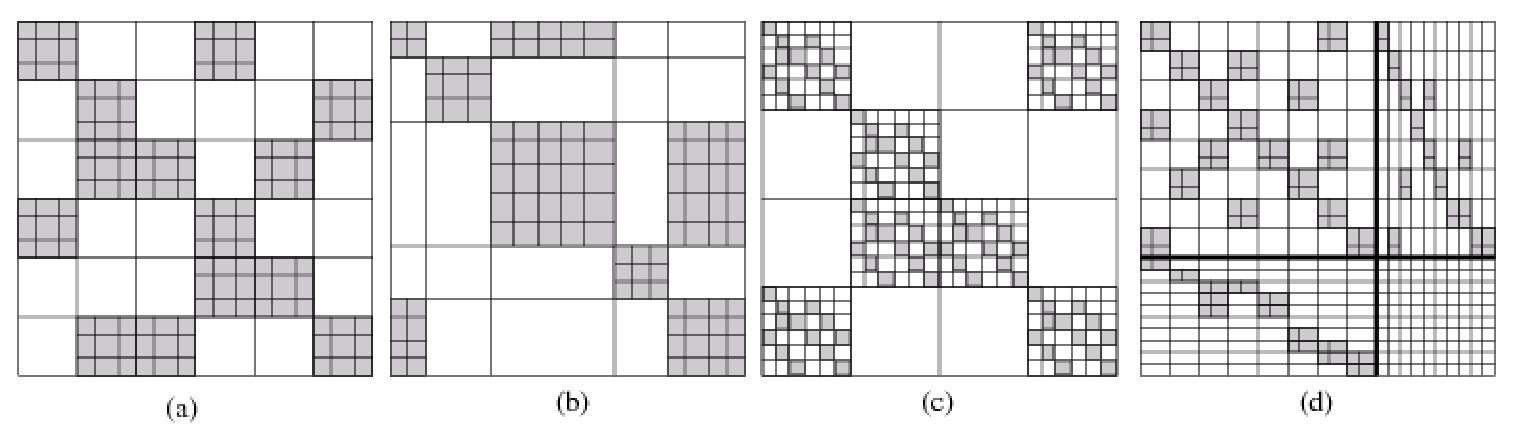
\epsfig{file=blockstructure, scale=0.485}
  \caption{Block structure of matrices arising in the finite element method}
  \label{fig:festructure}
\end{figure}
It is very important to note that this structure is typically known at
compile-time and this knowledge should be exploited to produce
efficient code. Moreover, block structuredness is recursive,
i.~e.~matrices are build from blocks which can themselves be build from
blocks. 

The Matrix Template Library also offers the possibility to partition a
matrix into blocks. However, their concept is top-down, i.~e.~an
already existing matrix is enriched by additional information to
implement the block structure. This is done at run-time and might thus
be less efficient and requires additional memory. In contrast the
bottom-up composition of block matrices from blocks can save memory.
We would like to stress that the library to be presented in this paper
is not nearly as broad in scope as the MTL.

\section{Vectors}

The interface of our vector classes is designed according to what they
represent from a mathematical point of view. The vector classes are
representations of vector spaces.

\subsection{Vector spaces}

In mathemetics vectors are elements of a vector space. A vector space
$V(\K)$, defined over a field $\K$, is a set of elements with two
operations: (i) vector space addition $+ : V\times V \to V$ and (ii) scalar
multiplication $* : \K\times V \to V$. These operations obey certain formal
rules, see your favourite textbook on linear algebra,
e.~g. \cite{LaBook}. In addition a 
vector space may be normed, i.~e.~there is a function (obeying certain
rules) $\|.\| : V \to \R$ which measures distance in the vector
space. Even more specialized vector spaces have a scalar product which
is a function $\cdot : V\times V \to \K$. 

How do you construct a vector space? The easiest way is to take a
field, such as $\K=\R$ or $\K=\C$ and take a tensor product:
\begin{equation*}
V = \K^n = \underbrace{\K\times\K\times\ldots\times\K}_{\text{$n$ times}}.
\end{equation*} 
$n\in\N$ is called the dimension of the vector space. There are also
infinite-dimensional vector spaceswhich are, however, not of interest
in the context here. The idea of tensor products can be generalized.
If we have vector spaces $V_1(\K),\ldots,V_n(\K)$ we can construct a
new vector space by setting
\begin{equation*}
V(\K) = V_1\times V_2 \times \ldots \times V_n.
\end{equation*} 
The $V_i$ can be \textit{any} vector space over the field $\K$. The
dimension of $V$ is the sum of the dimensions of the $V_i$. For a
a mathematician every finite-dimensional vector space is isomorphic to
the $\R^k$ for an appropriate $k$ but in our applications it is
important to know the difference between $(\R^2)^7$ and
$\R^{14}$. Having these remarks about vector spaces in mind we can now
turn to the class design.

\subsection{Vector classes}

ISTL provides the following classes to make up vector spaces:

\paragraph{FieldVector.}

The \lstinline!template<class K, int n> FieldVector<K,n>! class
template is used to represent a vector space
$V=\K^n$ where the field is given by the type
\lstinline!K!.  \lstinline!K! may be \lstinline!double!, \lstinline!float!,
\lstinline!complex<double>! or any other numeric type.
The dimension given by the template parameter
\lstinline!n! is assumed to be small. Members of this class are
implemented with template metaprograms to avoid tiny loops.
Example: Use \lstinline!FieldVector<double,2>! to define vectors with
a fixed dimension 2.

\paragraph{BlockVector.}

The \lstinline!template<class B> BlockVector<B>! class template builds
a vector space $V=B^n$ where the ``block type'' $B$ is given by the
template parameter \lstinline!B!. \lstinline!B! may be any other class
implementing the vector interface. The number of blocks $n$ is given
at run-time. Example: 
\begin{lstlisting}{}
BlockVector<FieldVector<double,2> >
\end{lstlisting}
can be used to define vectors of variable size where each block in turn
consists of two \lstinline!double! values.

\paragraph{VariableBlockVector.}
\label{class:varblockvec}

The \lstinline!template<class B> VariableBlockVector<B>! class
can be used to construct a vector space having a two-level
block structure of the form
$V=B^{n_1}\times B^{n_2}\times\ldots \times B^{n_m}$, i.e. it consists
of $m$ blocks $i=1,\ldots,m$ and each block in turn consists of $n_i$ blocks
given by the type \lstinline!B!. In principle this structure could be
built also with the previous classes but the implementation here is
more efficient. It allocates memory in one big array for all
components and for certain operations it is more efficient to
interpret the vector space as $V=B^{\sum_{i=1}^{m} n_i}$.

\subsection{Vectors are containers}

Vectors are containers over the base type \lstinline!K! or
\lstinline!B! in the sense of the Standard Template Library. Random
access is provided via \lstinline!operator[](int i)! where the indices
are in the range $0,\ldots,n-1$ with the number of blocks $n$ given by
the \lstinline!N! method. Here is a code fragment for illustration:
\begin{lstlisting}{}
typedef Dune::FieldVector<std::complex<double>,2> BType;
Dune::BlockVector<BType> v(20);
v[1] = 3.14;
v[3][0] = 2.56;
v[3][1] = std::complex<double>(1,-1);
\end{lstlisting}
Note how one \lstinline!operator[]()! is used for each level of block
recursion. 

Sequential access to container elements is provided via
iterators. Here is a generic function accessing all the elements of a
vector:
\begin{lstlisting}{}
template<class V> void f (V& v)
{
  typedef typename V::Iterator iterator;
  for (iterator i=v.begin(); i!=v.end(); ++i)
    *i = i.index();
  
  typedef typename V::ConstIterator const_iterator;
  for (const_iterator i=v.begin(); i!=v.end(); ++i)
    std::cout << (*i).two_norm() << std::endl;
}
\end{lstlisting}
The \lstinline!Iterator! class provides read/write access while the
\lstinline!ConstIterator! provides read-only access. The type names
are accessed via the \lstinline!::!-operator from the scope of the
vector class.

A uniform naming scheme enables writing of generic algorithms. The
following types are provided in the scope of any vector class:

\subsection{Operations}

A full list of all members of a vector class is given in Table
\ref{Tab:VectorMembers}. The norms are the same as defined for the
sparse BLAS standard \cite{BLASTForum}. The ``real'' variants avoid
the evaluation of a square root for each component in case of complex
vectors. The \lstinline!allocator_type! member type is explained below
in the section on memory management.

\begin{table}[htb]
\begin{center}
\begin{tabular}{|l|l|l|}
\hline
\textbf{expression} & \textbf{return type} & \textbf{note}\\
\hline
\hline
\texttt{X::field\_type} & T & T is assignable\\
\texttt{X::block\_type} & T & T is assignable\\
\texttt{X::allocator\_type} & T & see mem.~mgt.\\
\texttt{X::blocklevel} & \texttt{int} & block levels inside\\
\texttt{X::Iterator} & T & read/write access\\
\texttt{X::ConstIterator} & T & read-only access\\
\hline
\texttt{X::X()} & & empty vector \\
\texttt{X::X(X\&)} & & deep copy\\
\texttt{X::}$\sim$\texttt{X()} & & free memory\\
\texttt{X::operator=(X\&)} & \texttt{X\&} & \\
\texttt{X::operator=(field\_type\&)} & \texttt{X\&} & from scalar\\
\hline
\texttt{X::operator[](int)} & \texttt{field\_type\&} & \\
\texttt{X::operator[](int)} & \texttt{const field\_type\&} & \\
\texttt{X::begin()} & \texttt{Iterator} & \\
\texttt{X::end()} & \texttt{Iterator} & \\
\texttt{X::rbegin()} & \texttt{Iterator} & for reverse iteration \\
\texttt{X::rend()} & \texttt{Iterator} & \\
\texttt{X::find(int)} & \texttt{Iterator} & \\
\hline
\texttt{X::operator+=(X\&)} & \texttt{X\&} & $x = x+y$\\
\texttt{X::operator-=(X\&)} & \texttt{X\&} & $x = x-y$\\
\texttt{X::operator*=(field\_type\&)} & \texttt{X\&} & $x = \alpha x$\\
\texttt{X::operator/=(field\_type\&)} & \texttt{X\&} & $x = \alpha^{-1} x$\\
\texttt{X::axpy(field\_type\&,X\&)} & \texttt{X\&} & $x = x+\alpha y$\\
\texttt{X::operator*(X\&)} & \texttt{field\_type} & $x\cdot y$\\
\hline
\texttt{X::one\_norm()} & \texttt{double} & $\sum_i\sqrt{Re(x_i)^2+Im(x_i)^2}$\\
\texttt{X::one\_norm\_real()} & \texttt{double} &$\sum_i(|Re(x_i)|+|Im(x_i)|)$\\
\texttt{X::two\_norm()} & \texttt{double} &$\sqrt{\sum_i(Re(x_i)^2+Im(x_i)^2)}$\\
\texttt{X::two\_norm2()} & \texttt{double} &$\sum_i (Re(x_i)^2+Im(x_i)^2)$\\
\texttt{X::infinity\_norm()} & \texttt{double} &$\max_i\sqrt{Re(x_i)^2+Im(x_i)^2}$\\
\texttt{X::infinity\_norm\_real()} & \texttt{double} &$\max_i(|Re(x_i)|+|Im(x_i)|)$\\
\hline
\texttt{X::N()} & \texttt{int} & number of blocks\\
\texttt{X::dim()} & \texttt{int} & dimension of space\\
\hline
\end{tabular}
\end{center}

\caption{Members of a class \lstinline!X! conforming to the vector interface.}
\label{Tab:VectorMembers}
\end{table}

\subsection[Memory model]{Object memory model and memory management}

The memory model for all ISTL objects is deep copy as in the Standard
Template Library and in contrast to the Matrix Template
Library. Therefore, references must be used to avoid excessive copying
of objects. On the other hand temporary vectors with appropriate
structure can be generated simply with the copy constructor.



\subsection{Vector creation}

\section{Matrices}

\subsection{Linear mappings}

\subsection{Matrix classes}

For a matrix representing a linear map (or homomorphism) $A: V \mapsto
W$ from vector space $V$ to vector space $W$ the recursive block
structure of the matrix rows and columns immediatly follows
 from the recursive block structure of the vectors representing
the domain and range of the mapping, respectively. As a natural
consequence we designed the following matrix classes:

\paragraph{FieldMatrix.}
the \lstinline!template<class K, int n> FieldMatrix<K,n,m>! class
template is used to represent a linear map $M: V_1 \to V_2$ where
$V_1=\K^n$ and $V_2=\K^m$ are vector spaces over the field given by
template parameter \lstinline!K!. \lstinline!K! may be \lstinline!double!, \lstinline!float!,
\lstinline!complex<double>! or any other numeric type.
The dimensions of the two vector spaces  given by the template parameters
\lstinline!n! and \lstinline!m! are assumed to be small. The matrix is
stored as a dense matrix.
Example: Use \lstinline!FieldMatrix<double,2,3>! to define a linear
map from a vector space over doubles with dimension $2$ to one with
dimension $3$.

\paragraph{BCRSMatrix.}
The \lstinline!template<class B> BCRSMatrix! class template represents
a sparse matrix where the ``block type'' $B$ is given by the template
parameter \lstinline!B!. \lstinline!B! may be any other class
implementing the matrix interface.  The matrix class uses
a compressed row storage scheme.

\paragraph{VariableBCRSMatrix.}

The \lstinline!template<class B> VariableBCRSMatrix<B>! class can be
used to construct a linear map between two vector spaces having a two-level
block structure $V=B^{n_1}\times B^{n_2}\times\ldots \times B^{n_m}$
and $W=B^{m_1}\times B^{m_2}\times\ldots \times B^{m_k}$. Both are
represented by the 
\lstinline!template<class B> VariableBlockVector<B>! class,
see~\ref{class:varblockvec}. This is not implemented yet.

\subsection[Matrix containers]{Matrices are containers of containers}

Matrices are containers over the matrix rows. The matrix rows are
containers over the type  \lstinline!K! or
\lstinline!B! in the sense of the Standard Template Library. Random
access is provided via \lstinline!operator[](int i)! on the matrix to
the matrix rows and on the matrix rows to the matrix columns (if
present). Note that except for \lstinline!FieldMatrix!, which is a
dense matrix,  
\lstinline!operator[]! on the matrix row triggers a binary search for
the column.

For sequential access use 
\lstinline!RowIterator! and \lstinline!ColIterator! for read/write
access or  
\lstinline!ConstRowIterator! and \lstinline!ConstColIterator! for
readonly access to rows and columns, respectively. Here is a small example 
that prints the sparsity pattern of a matrix of type \lstinline!M!:

\begin{lstlisting}{}
typedef typename M::ConstRowIterator RowI;
typedef typename M::ConstColIterator ColI;
for(RowI row = matrix.begin(); row != matrix.end(); ++row){
  std::cout << "row "<<row.index()<<": "
  for(ColI col = row->begin(); col != row->end(); ++col)
    std::cout<<col.index()<<" ";
  std::cout<<std::endl;
}
\end{lstlisting}

\subsection{Precision control}

\subsection{Operations}

As with the vector interface a uniform naming convention enables
generic algorithms. See Table \ref{Tab:MatrixMembers} for a
complete list of names.
\begin{table}[htb]
\begin{center}
\begin{tabular}{|l|l|l|}
\hline
\textbf{expression} & \textbf{return type} & \textbf{note}\\
\hline
\hline
\texttt{M::field\_type} & T & T is assignable\\
\texttt{M::block\_type} & T & T is assignable\\
\texttt{M::row\_type} & T & a T is assignable\\
\texttt{M::allocator\_type} & T & see mem.~mgt.\\
\texttt{M::blocklevel} & \texttt{int} & block levels inside\\
\texttt{M::RowIterator} & T & over rows\\
\texttt{M::ColIterator} & T & over columns\\
\texttt{M::ConstRowIterator} & T & over rows\\
\texttt{M::ConstColIterator} & T & over columns\\
\hline
\texttt{M::M()} & & empty matrix \\
\texttt{M::M(M\&)} & & deep copy\\
\texttt{M::}$\sim$\texttt{M()} & & free memory\\
\texttt{M::operator=(M\&)} & \texttt{M\&} & \\
\texttt{M::operator=(field\_type\&)} & \texttt{M\&} & from scalar\\
\hline
\texttt{M::operator[](int)} & \texttt{row\_type\&} & \\
\texttt{M::operator[](int)} & \texttt{const row\_type\&} & \\
\texttt{M::begin()} & \texttt{RowIterator} & \\
\texttt{M::end()} & \texttt{RowIterator} & \\
\texttt{M::rbegin()} & \texttt{RowIterator} & reverse iteration\\
\texttt{M::rend()} & \texttt{RowIterator} & \\
\hline
\texttt{M::operator*=(field\_type\&)} & \texttt{M\&} & $A = \alpha A$\\
\texttt{M::operator/=(field\_type\&)} & \texttt{M\&} & $A = \alpha^{-1} A$\\
\hline
\texttt{M::umv(X\& x,Y\& y)}    &  & $y = y + Ax$\\
\texttt{M::mmv(X\& x,Y\& y)}    &  & $y = y - Ax$\\
\texttt{M::usmv(field\_type\&,X\& x,Y\& y)}   &  & $y = y + \alpha Ax$\\
\texttt{M::umtv(X\& x,Y\& y)}   &  & $y = y + A^Tx$\\
\texttt{M::mmtv(X\& x,Y\& y)}   &  & $y = y - A^Tx$\\
\texttt{M::usmtv(field\_type\&,X\& x,Y\& y)}  &  & $y = y + \alpha A^Tx$\\
\texttt{M::umhv(X\& x,Y\& y)}   &  & $y = y + A^Hx$\\
\texttt{M::mmhv(X\& x,Y\& y)}   &  & $y = y - A^Hx$\\
\texttt{M::usmhv(field\_type\&,X\& x,Y\& y)}  &  & $y = y + \alpha A^Hx$\\
\hline
\texttt{M::solve(X\& x,Y\& b)}   &  & $x = A^{-1}b$\\
\texttt{M::inverse(M\& B)} & & $B=A^{-1}$\\
\texttt{M::leftmultiply(M\& B)} & \texttt{M\&} & $A = BA$\\
\hline
\texttt{M::frobenius\_norm()} & \texttt{double} & see text\\
\texttt{M::frobenius\_norm2()} & \texttt{double} &see text\\
\texttt{X::infinity\_norm()} & \texttt{double} & see text\\
\texttt{X::infinity\_norm\_real()} & \texttt{double} &see text\\
\hline
\texttt{M::N()} & \texttt{int} & row blocks\\
\texttt{M::M()} & \texttt{int} & col blocks\\
\texttt{M::rowdim(int)} & \texttt{int} & dim.~of row block\\
\texttt{M::rowdim()} & \texttt{int} & dim.~of row space\\
\texttt{M::coldim(int)} & \texttt{int} & dim.~of col block\\
\texttt{M::coldim()} & \texttt{int} & dim.~of col space\\
\texttt{M::exists(int i, int j)} & \texttt{bool} &\\
\hline
\end{tabular}
\end{center}

\caption{Members of a class \lstinline!M! conforming to the matrix
  interface. \lstinline!X! and \lstinline!Y! are any vector classes.}
\label{Tab:MatrixMembers}
\end{table}

\subsection{Matrix creation}

\section{Algorithms}

\subsection{Input/output}

\subsection{Block recursion}

The basic feature of the concept described by the matrix and vector
classes, is their recursive block structure. Let $A$ be a
matrix with blocklevel $l>1$ then each block $A_{ij}$ can be treated
as (or actually is) a matrix itself. This recursiveness can be
exploited in generic algorithm using the defined
\lstinline!block_level! of the matrix and vector classes.

Most preconditioner can be modified to honor this recursive
structure for a specific number of block levels $k$. They then work as
normal on the offdiagonal blocks, treating them as traditional matrix
entries. For the diagonal values a special procedure applies:  If
$k>1$ the diagonal is treated as a matrix itself and the preconditioner
is applied recursively on the matrix representing the diagonal value
$D=A_{ii}$ with blocklevel $k-1$. For the case that $k=1$ the diagonal
is treated as a 
matrix entry resulting in a linear solve or an identity operation
depending on the algorithm. 

\subsection{Triangular solves}

In the formulation of most iterative methods upper and lower
triangular and diagonal solves play an important role. 
ISTL provides block recursive versions of these generic 
building blocks using template metaprogramming, see Table
\ref{Tab:TriangularSolves} for a listing of these methods. In the table matrix
$A$ is decomposed into $A=L+D+U$, where $L$ is a strictly lower block
triangular, $D$ is a block diagonal and $U$ is a strictly upper block
triangular matrix. An arbitrary block recursion level can be given by an
additional parameter. If this parameter is omitted it defaults to $1$.

\begin{table}[htb]
\begin{center}
\begin{tabular}{|l|l|}
\hline
\textbf{function} & \textbf{computation}\\
\hline
\hline
\texttt{bltsolve(A,v,d)}  & $v=(L+D)^{-1}d$\\
\texttt{bltsolve(A,v,d,$\omega$)}  & $v=\omega(L+D)^{-1}d$\\
\texttt{ubltsolve(A,v,d)}  & $v=L^{-1}d$\\
\texttt{ubltsolve(A,v,d,$\omega$)}  & $v=\omega L^{-1}d$\\
\hline
\texttt{butsolve(A,v,d)}  & $v=(D+U)^{-1}d$\\
\texttt{butsolve(A,v,d,$\omega$)}  & $v=\omega(D+U)^{-1}d$\\
\texttt{ubutsolve(A,v,d)}  & $v=U^{-1}d$\\
\texttt{ubutsolve(A,v,d,$\omega$)}  & $v=\omega U^{-1}d$\\
\hline
\texttt{bdsolve(A,v,d)}  & $v=D^{-1}d$\\
\texttt{bdsolve(A,v,d,$\omega$)}  & $v=\omega D^{-1}d$\\
\hline
\end{tabular}
\end{center}

\caption{Functions available for block triangular and block diagonal
  solves. The matrix $A$ is decomposed into $A=L+D+U$ where $L$ is
  strictly lower block triangular, $D$ is block diagonal and $U$ is
  strictly upper block triangular. Standard is one level of block
  recursion, arbitrary level can be given by additional parameter.}
\label{Tab:TriangularSolves}
\end{table}

\subsection{Simple iterative solvers}

Using the same block recursive template metaprogramming technique,
kernels for the defect formulations of simple iterative solvers are
available in ISTL. The number of block recursion
levels can again be given as an additional argument. See
Table \ref{Tab:IterativeSolvers} for a list of these kernels.
\begin{table}[htb]
\begin{center}
\begin{tabular}{|l|l|}
\hline
\textbf{function} & \textbf{computation}\\
\hline
\hline
\texttt{dbjac(A,x,b,$\omega$)}  & $x=x+\omega D^{-1}(b-Ax)$ \\
\texttt{dbgs(A,x,b,$\omega$)}   & $x = x + \omega (L+D)^{-1}(b-Ax)$\\
\texttt{bsorf(A,x,b,$\omega$)}  & $x^{k+1}_i = x^k_i + \omega
A_{ii}^{-1}\left [
  b_i - \sum\limits_{j<i} A_{ij}x^{k+1}_j - \sum\limits_{j\geq i}
  A_{ij}x^{k}_j\right ]$\\
\texttt{bsorb(A,x,b,$\omega$)}  & $x^{k+1}_i = x^k_i + \omega
A_{ii}^{-1}\left [
  b_i - \sum\limits_{j\leq i} A_{ij}x^{k}_j - \sum\limits_{j>i}
  A_{ij}x^{k+1}_j\right ]$\\
\hline
\end{tabular}
\end{center}

\caption{Kernels for iterative solvers. 
  The matrix $A$ is decomposed into $A=L+D+U$ where $L$ is
  strictly lower block triangular, $D$ is block diagonal and $U$ is
  strictly upper block triangular. Standard is one level of block
  recursion, arbitrary level can be given by additional parameter.}
\label{Tab:IterativeSolvers}
\end{table}

\subsection{Sparse LU decomposition}

\section{Solver Interface}
\label{sec:solver-interface}

The solvers in ISTL do not work on matrices directly. Instead we use
an abstract Operator concept. Thus we can even model and solve linear
maps that are not stored as matrices (e.~g. on the fly computed linear
operators).

\subsection{Operators}
\label{sec:operators}


{\lstset{breaklines=true}
The base class
\lstinline!template<class X, class Y> LinearOperator! represents
linear maps. The 
template parameter \lstinline!X! is the type of the domain and
\lstinline!Y! is the type of the range of the operator.  A linear
operator provides the methods \lstinline!apply(const X& x, Y& y)! and 
apply \lstinline!applyscaledadd(const X& x, Y& y)! performing the
operations $y = A(x)$ and $y = y + \alpha A(x)$, respectively.
The subclass 
\lstinline!template<class M, class X, class Y> AssembledLinearOperator!
represents linear operators that have a matrix
representation. Convertion from any matrix into a linear operator is
done by the class 
\lstinline!template<class M, class X, class Y> MatrixAdapter!.

\subsection{Scalarproducts}
\label{sec:scalarproducts}

For convergence tests and the stopping criteria Krylow methods need to
compute scalar products and norms on the underlying vector spaces. The
base class \lstinline!template<class X> Scalarproduct! provides
methods \lstinline!field_type dot(const X& x, const X&y)! and
\lstinline!double norm(const X& x)! to calculate these. For
sequential programs use 
\lstinline!template<class X> SeqScalarProduct! which simply maps this
to functions of the vector implementations.

\subsection{Preconditioners}
\label{sec:preconditioners}


The \lstinline!template<class X, class Y> Preconditioner! provides the
abstract base class for all precondioners in ISTL. The method
\lstinline!void pre(X& x, Y& b)! has to be called before applying the
preconditioner. Here \lstinline!x! is the left hand side and
\lstinline!b! is the right hand side of the operator equation. The
method may, e.~g. scale the system, allocate memory or compute an (I)LU
decomposition. The method \lstinline!void apply(X& v, const Y&)!
applies one step of the preconditioner to the system $A(\vec v)=\vec d$.
Here \lstinline!b! should contain the current defect and
\lstinline!v! should be $0$. Upon exit of the method \lstinline!v!
contains the computed update to
the current guess, i.~e. $\vec v = M^{-1} \vec
d$ where $M$ is the approximate inverse of the operator $A$
characterizing the preconditioner. The method \lstinline!void post(X& x)!
should be called after all computations to give the precondtioner the
chance to clean allocated resources. 

See Table \ref{tab:precond} for a list of available
preconditioner. 
\begin{table}[htb]
  \centering
  \caption{Preconditioners}
  \label{tab:precond}
  \begin{tabular}{|l|l|c|c|}
    \hline
    \textbf{class} & \textbf{implements}&\textbf{s/p}& \textbf{recursive}\\\hline\hline
    \lstinline!SeqJac! & Jacobi method& s & x\\
    \lstinline!SeqSOR! & successive overrelaxation (SOR) & s& x\\
    \lstinline!SeqSSOR! & symmetric SSOR & s&x\\
    \lstinline!SeqILU! & incomplete LU decomposition (ILU)& s&\\
    \lstinline!SeqILUN! & ILU decpmposition of order N &s&\\
    \lstinline!Pamg::AMG! & algebraic multigrid method &s/p&\\
    \lstinline!BlockPreconditioner!& Additive overlapping Schwarz&p&\\\hline
  \end{tabular}
\end{table}
They have the template parameters \lstinline!M!
representing the type of the matrix they work on, \lstinline!X!
representing the type of the domain, \lstinline!Y! representing the
type of the range of the linear system. The block recursive
preconditioner are marked with ``x'' in the last column. For them the
recursion depth is specified via an additional template parameter
\lstinline!int l!. The column labeled ``s/p''
specifies whether they support {\bf s}equential and/or {\bf p}arallel
mode.

\subsection{Solvers}
\label{sec:solvers}

All solvers are subclasses of the abstract base class
\lstinline!template<class X, class Y> InverseOperator! representing
the inverse of an operator from the domain of type \lstinline!X! to
the range of type \lstinline!Y!. The actual solve of the system
$A(\vec x)=\vec b$ is done in the method 
\lstinline!void apply(X& x, Y& b, InverseOperatorResult& r)!. In the
\lstinline!InverseOperatorResult! some statistics about the solution
process, e.~g. iteration count, achieved defect reduction, etc., are
stored.
All solvers only use methods of instances of
\lstinline!LinearOperator!, \lstinline!ScalarProduct! and
\lstinline!Preconditioner!. These are provided in the constructor.

See Table \ref{tab:solvers} for a list of available solvers. All
solvers are template classes with a template parameter \lstinline!X!
providing them with the vector implementation used.
\begin{table}[htb]
  \centering
  \caption{ISTL Solvers}
  \label{tab:solvers}
  \begin{tabular}{|l|l|}
\hline
    \textbf{class}&\textbf{implements}\\\hline\hline
    \lstinline!LoopSolver!& only apply precoditioner multiple time\\
    \lstinline!GradientSolver!& preconditioned radient method\\
    \lstinline!CGSolver!&preconditioned conjugate gradient method\\
    \lstinline!BiCGStab!&preconditioned biconjugate gradient stabilized method\\\hline
  \end{tabular}
\end{table}
\subsection{Parallel Solvers}
\label{sec:parallelism}

Instead of using parallel data structures (matrices and vectors) that
(implicitly) know the data distribution and communication patterns
like in PETSc \cite{petsc-web-page,petsc-user-ref} we decided to
decouple the parallelization from the data structures used. Basically
we provide an abstract consistency model on top of our linear
algebra. This is hidden in the parallel implementations of the interfaces
of \lstinline!LinearOperator!,
\lstinline!Scalarproduct! and \lstinline!Preconditioner!, which assure
consistency of the data (by communication) for the \lstinline!InverseOperator!
implementation. Therefore the same Krylow method algorithms work in
parallel and sequential mode. 

Based on the idea proposed in \cite{dddalg} we implemented parallel overlapping
Schwarz preconditioners with inexact (sequential) subdomain solvers and a
parallel algebraic multigrid preconditioner
together with appropriate implementations of
\lstinline!LinearOperator! and
\lstinline!Scalarproduct!. Nonoverlapping versions are currently being
worked on.

Note that using this approach it easy two switch form the currently
implemented MPI version to new parallel programming paradigms that
might be needed on new platforms.


\section{Performance}
We evaluated the performance of our implementation on a Petium 4 Mobile
2.4 GHz with a measured memory bandwith of 1084 MB/s for the daypy
operation ($x = y + \alpha z$) in Tables
\ref{tab:istl_performance}. 
\begin{table}[htb]
  \centering
  \caption{Performance Tests}
  \label{tab:istl_performance}
  \mbox{\small
    \subtable[scalar product]{\label{tab:perf_sp}
      \begin{tabular}{lrrrrr}
          \hline
          \hline
          $N$ & 500 & 5000 & 50000 & 500000 & 5000000 \\
          \hline
          MFLOPS & 896 & 775 & 167 & 160 & 164 \\
          \hline
          \hline
        \end{tabular}}
    \subtable[daxpy operation $y = y + \alpha x$]{\label{tab:perf_daxpy}
      \begin{tabular}{rrrrr}
        \hline
        \hline
         500 & 5000 & 50000 & 500000 & 5000000 \\
        \hline
        936 & 910 & 108 & 103 & 107 \\
        \hline
        \hline
      \end{tabular}}}
  \mbox{\small
    \subtable[Matrix-vector product, %\lstinline!BCRSMatrix!,
    5-point stencil, $b$: block size]{\label{tab:perf_mvp}
      \begin{tabular}{lrrrrr}
        \hline
        \hline
        $N,b$ & 100,1 & 10000,1 & 1000000,1 & 1000000,2 & 1000000,3\\
        \hline
        MFLOPS & 388 & 140 & 136 & 230 & 260\\
        \hline
        \hline
      \end{tabular}}
    \subtable[Damped Gau\ss{}--Seidel]{\label{tab:perf_gs}
      \begin{tabular}{rrr}
          \hline
          \hline
          & \mbox{C } & ISTL\\
          \hline
          time / it. [s] & 0.17 & 0.18\\
          \hline
          \hline
        \end{tabular}}}
\end{table}
The code was comiled with the GNU C++ 
compiler version 4.0 with -O3 optimization. In the tables $N$ is the
number of 
unknown blocks (equals the number of unknows for the scalar cases in
Tables \ref{tab:perf_sp}, \ref{tab:perf_daxpy}, \ref{tab:perf_gs}).
The performance for the scalarproduct,
see Table \ref{tab:perf_sp},
and the daxpy operation, see Table \ref{tab:perf_daxpy}  is nearly
optimal and for large $N$ the limiting factor is clearly the memory
bandwith. Table \ref{tab:perf_mvp} shows that we take advantage of
cache reusage for matrices of dense blocks with block size $b>1$.
In Table
\ref{tab:perf_gs} we compared the generic implementation of
the Gau\ss{}--Seidel solver in ISTL with a specialized C
implementation. The measured times per iteration show that there is
now lack of computational efficiency due to the generic implementation. 

% bibtex bibliography
\bibliographystyle{plain}
\bibliography{istl.bib}

% some links
% http://www.netlib.org/blas/blast-forum/
% http://www.osl.iu.edu/research/mtl/
% http://www.osl.iu.edu/research/itl/ (based on MTL, mostly Krylov)
% http://netlib.org/utk/people/JackDongarra/la-sw.html
% the last one: FREELY AVAILABLE SOFTWARE FOR
% LINEAR ALGEBRA ON THE WEB (May 2004) by Jack Dongarra
% http://www.oonumerics.org/blitz/

\end{document}
